\section{Formal Analysis}
\subsection{Alloy Code}
\begin{lstlisting}[language=alloy]
//SIGNATURES

abstract sig Account {
 	name: one Name,
  	surname: one Surname,
  	username: one Username,
  	email: one Email,
  	password: one Password
}

sig Name {
}{
  	no n : Name | n. ~name  = none
}

sig Surname {
}{
  	no s : Surname  | s. ~surname = none
}

sig Email {}
{
  	no disj a1, a2 : Account | a1.email = a2.email
  	no e: Email | e. ~email = none
}

sig Username {}
{
  	no disj a1, a2 : Account | a1.username = a2.username
 	no u: Username | u.~username = none
}

sig Password {
} {
	no p: Password | p. ~password = none
}

sig Farm {
	area: one Area
} {
 	#this.~inspection >= 2
	no f:Farm | f.~farm = none
	no f:Farm | f.~farms_dashboard = none
}

sig Post {
} {
	no p: Post | p.~posts = none
}

sig DailyPlan {
  visits: set Visit
}{
	no d:DailyPlan | d.~dailyplan = none
}

sig Visit {
	inspection: one Farm
}  {
	no v:Visit | v.~visits = none
}

one sig DashBoard {
	farms_dashboard: set Farm
}

sig Thread {
	posts: some Post,
} {
	no  t:Thread| t.~threads = none
}

one sig Forum {
  	threads: set Thread,
}

sig Area {
}

sig PolicyMaker extends Account {
  	dashboard: one DashBoard,
}

sig Farmer extends Account {
 	farm: one Farm,
  	forumF: one Forum,
  	requests : set HelpRequest
}

sig Agronomist extends Account {
  	forumA: one Forum,
  	areas: one Area,
  	dashboard: one DashBoard,
  	dailyplan: one DailyPlan
}

sig HelpRequest{
  	agronomist : one Agronomist
}{
  	no h: HelpRequest | h. ~requests = none
}


----------------------------------------------------------------------
//FACTS

//This fact ensures that a post is created by only one thread
fact aboutThread {
	all disj t1,t2: Thread| t1.posts & t2.posts = none
}

//This fact ensures that every farmer owns a farm
fact aboutFarms {
	no disj f1,f2: Farmer | f1.farm = f2.farm
}

//This fact contains constraints regarding agronomists:
	// - every agronomist owns a different area
	// - every agronomist has a different daily plan
	// - no visit belongs to different daily plans
fact aboutAgron {
	no disj a1, a2: Agronomist | a1.areas = a2.areas
	no disj a1, a2: Agronomist | a1.dailyplan = a2.dailyplan
	all disj d1,d2: DailyPlan | (d1.visits=none and d2.visits=none) or (d1.visits & d2.visits = none)
}

//This fact ensures that any farm belongs to different areas
fact aboutArea {
	all disj a1,a2: Area |  (a1.~area=none and a2.~area=none) or (a1.~area & a2.~area = none)
}

//This fact ensures that every daily plan owns visits to farmer belonging to the corresponding agronomist
fact aboutDailyPlan{
	all d:DailyPlan | (d.visits.inspection.area != none) implies (d.visits.inspection.area = d.~dailyplan.areas)
}

//This fact contains constraints regarding help requests:
	// - every help requests can be sent only to the corresponding agronomist
	// - every farmer sends different requests
fact aboutHelpRequest{
  	all h: HelpRequest | h.agronomist.areas = h. ~requests.farm.area
  	all disj f1, f2: Farmer | f1.requests & f2.requests = none
}


----------------------------------------------------------------------
//ASSERTS

assert agronomistArea {
  	no disj a1, a2: Agronomist | {
    		a1.areas = a2.areas
  	}
}

assert helpRequest {
  	all a1, a2: Agronomist, f: Farmer, disj h1, h2: HelpRequest | {
    		(h1.~requests = f and h2.~requests = f and a1.~agronomist = h1 and a2.~agronomist = h2) implies (a1=a2)
  	}
}

assert dailyPlan {
  	all a1, a2: Area, disj v1, v2: Visit | {
    		(v1.inspection.area = a1 and v2.inspection.area = a2 and v1.~visits.~dailyplan = v2.~visits.~dailyplan) implies (a1 = a2)
  	}
}


----------------------------------------------------------------------
//PREDICATES

//A simulation that shows the daily plan of Agronomists w/ visits to Farmer of
//their area of responsibility
pred world1 {
	#Farmer = 3
	#Agronomist = 2
	#PolicyMaker = 0
	#Thread = 0
	#Post = 0
}
//run world1 for 6

//A simulation that shows the functioning of the dashboard
pred world2{
	#PolicyMaker = 2
	#Agronomist = 2
	#Farmer = 1
	#Visit = 2
}

//A simulation that shows the different types of help given to the farmers
pred world3{
	#Farmer = 3
	#Agronomist = 3
	#PolicyMaker = 0
	#Thread = 3
}

//A simulation that shows the registration
pred world4{
	#Farmer = 1
	#PolicyMaker = 1
	#Agronomist = 1
}

run world4 for 3


check agronomistArea for 10
check helpRequest for 10
check dailyPlan for 10


run world1 for 6
run world2 for 5
run world3 for 6
run world4 for 3

\end{lstlisting}

\newpage

\begin{figure}[H]
	\centering
	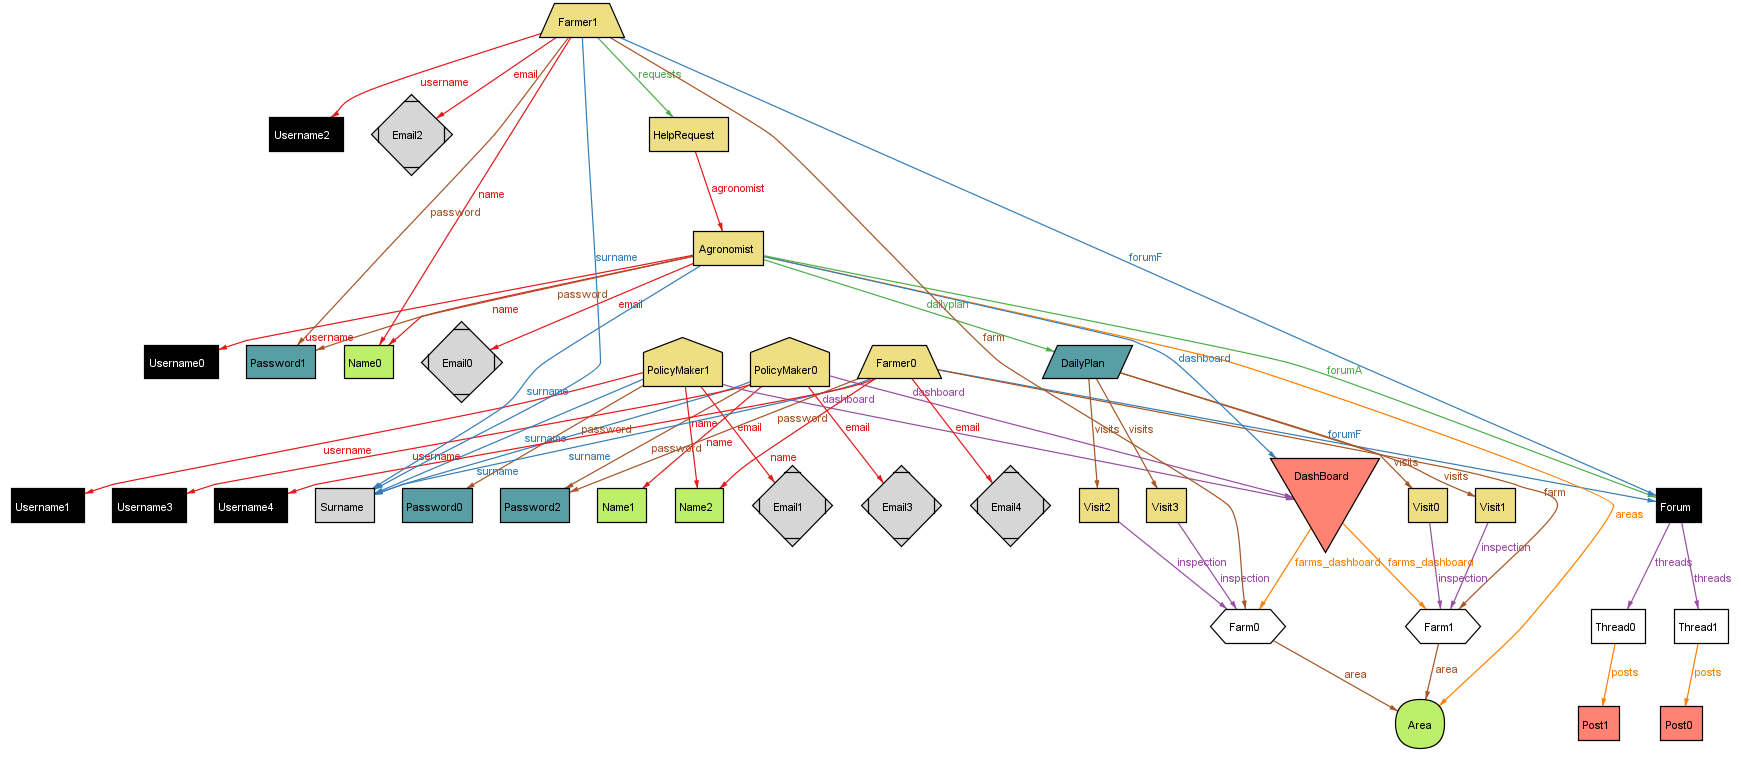
\includegraphics[angle=90, scale=0.6]{Images/completeWorld.png}
	\caption{All the elements managed in the alloy analysis}
\end{figure}

\newpage

\begin{figure}[H]
	\centering
	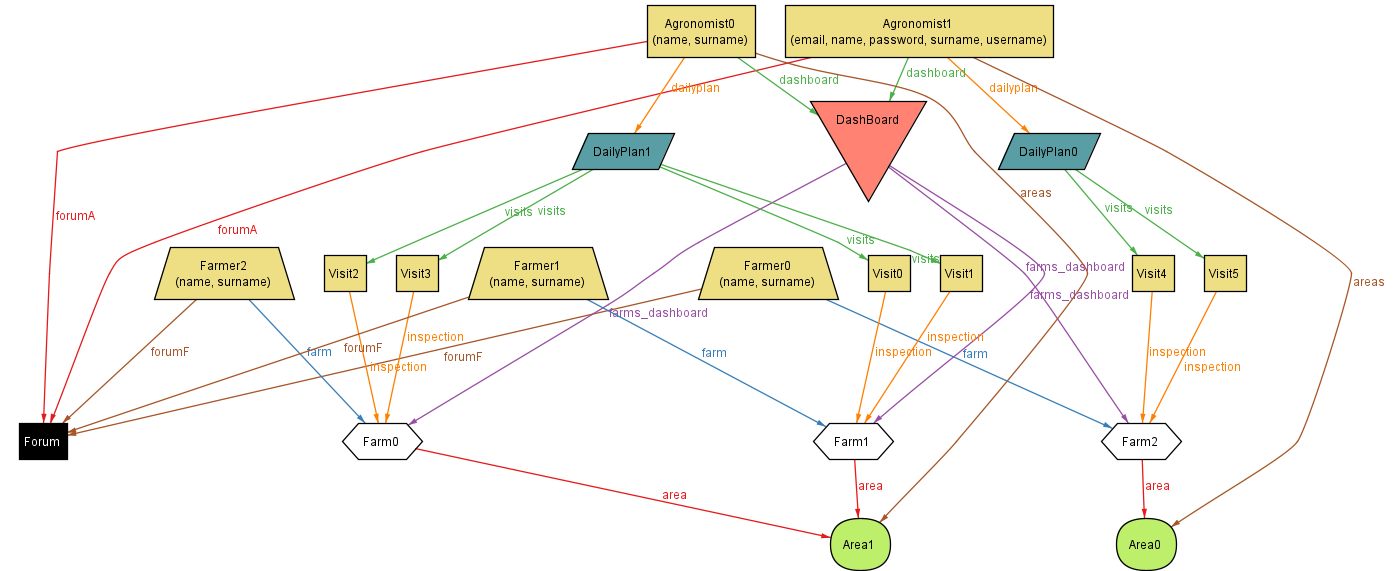
\includegraphics[angle=90, scale=0.45]{Images/world1.png}
	\caption{Representation of the execution of predicate world1}
\end{figure}

\newpage

\begin{figure}[H]
	\centering
	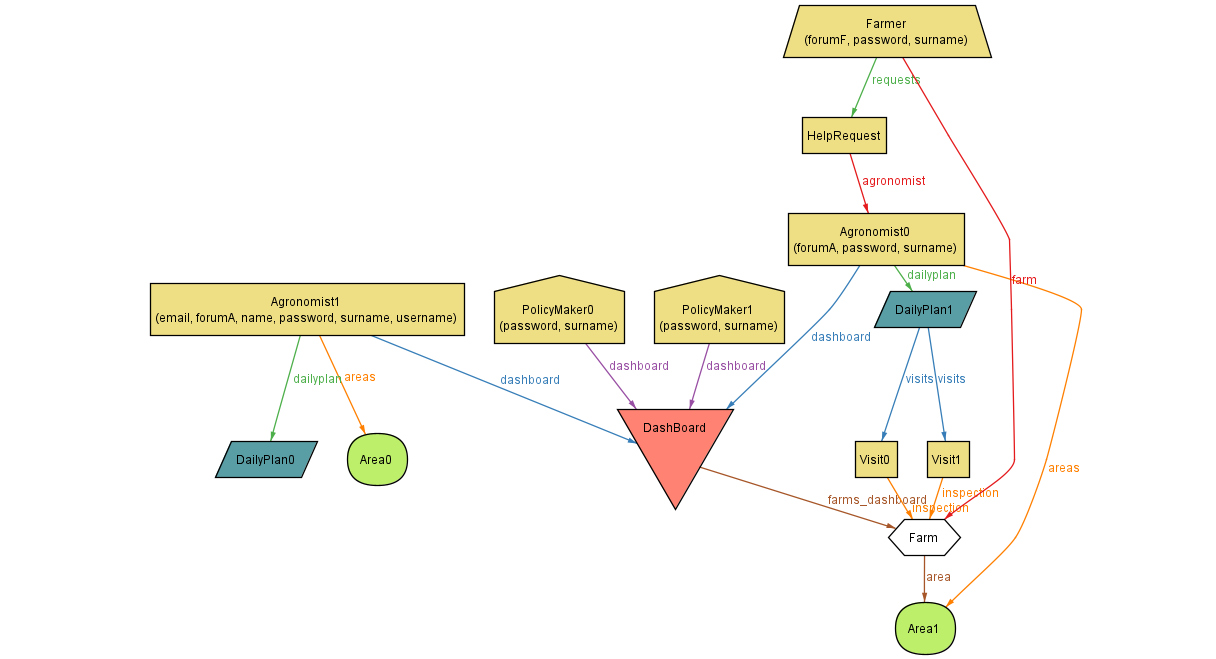
\includegraphics[angle=90, scale=0.5]{Images/world2.png}
	\caption{Representation of the execution of predicate world2}
\end{figure}

\newpage

\begin{figure}[H]
	\centering
	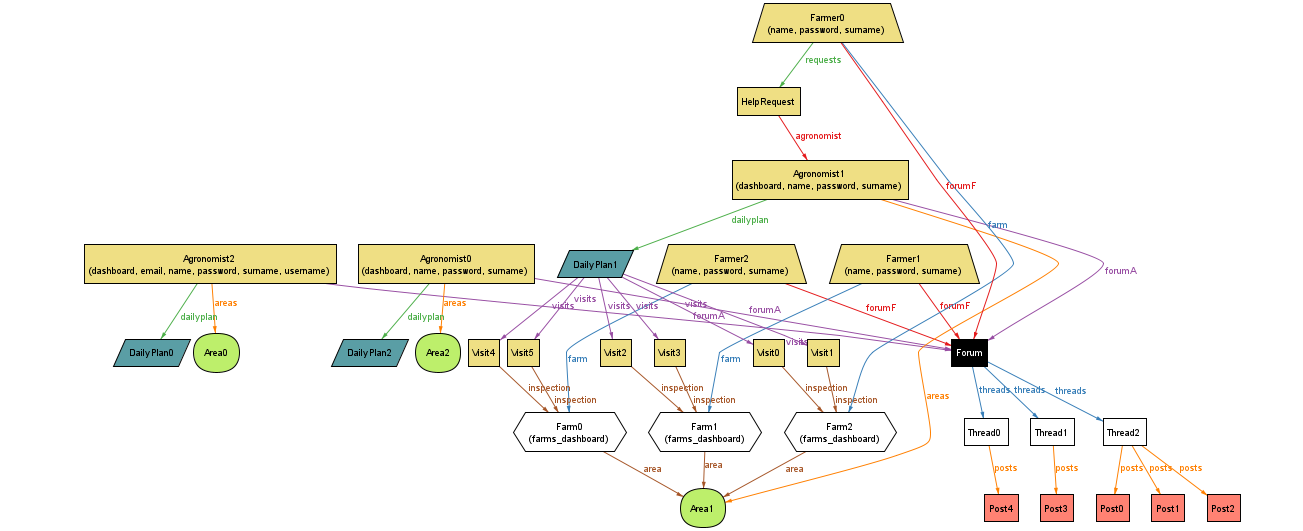
\includegraphics[angle=90, scale=0.47]{Images/world3.png}
	\caption{Representation of the execution of predicate world3}
\end{figure}

\newpage

\begin{figure}[H]
	\centering
	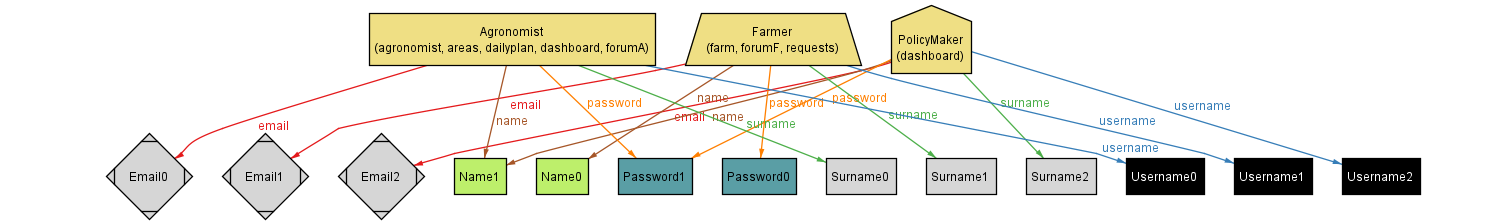
\includegraphics[angle=90, scale=0.43]{Images/world4.png}
	\caption{Representation of the execution of predicate world4}
\end{figure}